En este apartado se define el diseño de las clases que componen el sistema desarrollado. 
En primer lugar, se presenta el diagrama de paquetes, que muestra la estructura de los paquetes que componen el sistema.
Posteriormente, se presenta el diagrama de clases, que muestra las clases que componen el sistema y las relaciones entre ellas así como una descripción.

\subsection{Diagrama de paquetes} 
El sistema se divide en dos paquetes principales:
\begin{itemize}
    \item \textbf{restapi}: se corresponde con el \textit{backend} del sistema, contiene las clases que implementan la API REST del sistema y la lógica de negocio.
    \item \textbf{frontend}: se corresponde con el \textit{frontend} del sistema, contiene las clases que implementan la interfaz de usuario.
\end{itemize}

En la \coloredUnderline{\hyperlink{fig:6_5_Diagrama-Paquetes}{Figura \ref*{fig:6_5_Diagrama-Paquetes}: \nameref*{fig:6_5_Diagrama-Paquetes}}} se muestra el diagrama de paquetes del sistema.
\begin{figure}[H]
    \hypertarget{fig:6_5_Diagrama-Paquetes}{}
    \centering
    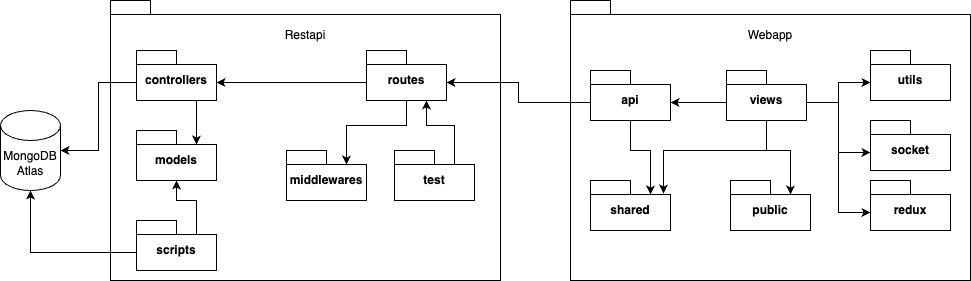
\includegraphics[width=0.8\linewidth]{figures/6-Analisis/6-Clases/6_5-vista_general-paquetes.png}
    \caption{Diagrama de Paquetes del Sistema}
    \label{fig:6_5_Diagrama-Paquetes}
\end{figure}

\subsection{Descripción de los Paquetes}
\subsubsection{restapi}
El paquete \textbf{restapi} contiene las clases que implementan la API REST del sistema y la lógica de negocio. Este paquete se divide en los siguientes subpaquetes:
\begin{itemize}
    \item \textbf{controllers}: contiene las clases que implementan los controladores de la API REST, se encargan de gestionar las peticiones HTTP y las respuestas. Se comunica con la base de datos.
    \item \textbf{models}: contiene las clases que implementan los modelos de datos del sistema.
    \item \textbf{routes}: contiene las clases que implementan las rutas de la API REST, se encargan de definir las rutas y los métodos HTTP asociados.
    \item \textbf{middlewares}: contiene las clases que implementan los middlewares de la API REST, se encargan de gestionar la autenticación y la autorización de los usuarios.
    \item \textbf{scripts}: contiene las clases que implementan los scripts de inicialización de la base de datos.
    \item \textbf{tests}: contiene las clases que implementan las pruebas unitarias de las clases de los otros subpaquetes.
\end{itemize}


\subsubsection{frontend}
El paquete \textbf{frontend} contiene las clases que implementan la interfaz de usuario. Este paquete se divide en los siguientes subpaquetes:
\begin{itemize} 
    \item \textbf{src}: contiene las clases que implementan la lógica de la interfaz de usuario.
    \begin{itemize}
        \item \textbf{api}: contiene las clases que implementan la API del frontend, se encargan de gestionar las peticiones HTTP/HTTPS al backend.
        \item \textbf{views}: contiene las clases que implementan las vistas de la interfaz de usuario. A su vez, se divide en los siguientes subpaquetes:
        \begin{itemize}
            \item \textbf{components}: contiene las clases que implementan los componentes de la interfaz de usuario.
            \item \textbf{pages}: contiene las clases que implementan las páginas de la interfaz de usuario.
        \end{itemize}
        \item \textbf{redux}: contiene las clases que implementan los estados de Redux.
        \item \textbf{socket}: contiene las clases que implementan la conexión con Socket.io.
        \item \textbf{shared}: contiene las clases que implementan los tipos de datos compartidos entre las distintas partes de la interfaz de usuario.
        \item \textbf{utils}: contiene las clases que implementan utilidades de la interfaz de usuario.
    \end{itemize}
    \item \textbf{public}: contiene los archivos estáticos de la interfaz de usuario.
    \item \textbf{tests}: contiene las clases que implementan las pruebas de la interfaz de usuario.
\end{itemize}

\subsection{Diagrama de Clases} 
El diagrama de clases muestra las clases que componen la lógica de negocio del sistema. Se omite representar las relaciones entre las clases para simplificar el diagrama y que sea más legible. En el apartado \coloredUnderline{\hyperlink{sec:6_6_3-Descripcion-Clases}{ \ref*{sec:6_6_3-Descripcion-Clases}: \nameref*{sec:6_6_3-Descripcion-Clases}}}
se describen las clases y las relaciones entre ellas.

En la \coloredUnderline{\hyperlink{fig:6_6_Diagrama-Clases}{Figura \ref*{fig:6_6_Diagrama-Clases}: \nameref*{fig:6_6_Diagrama-Clases}}} se muestra el diagrama de clases del paquete \textbf{restapi}.
\begin{figure}[H]
    \hypertarget{fig:6_6_Diagrama-Clases}{}
    \centering
    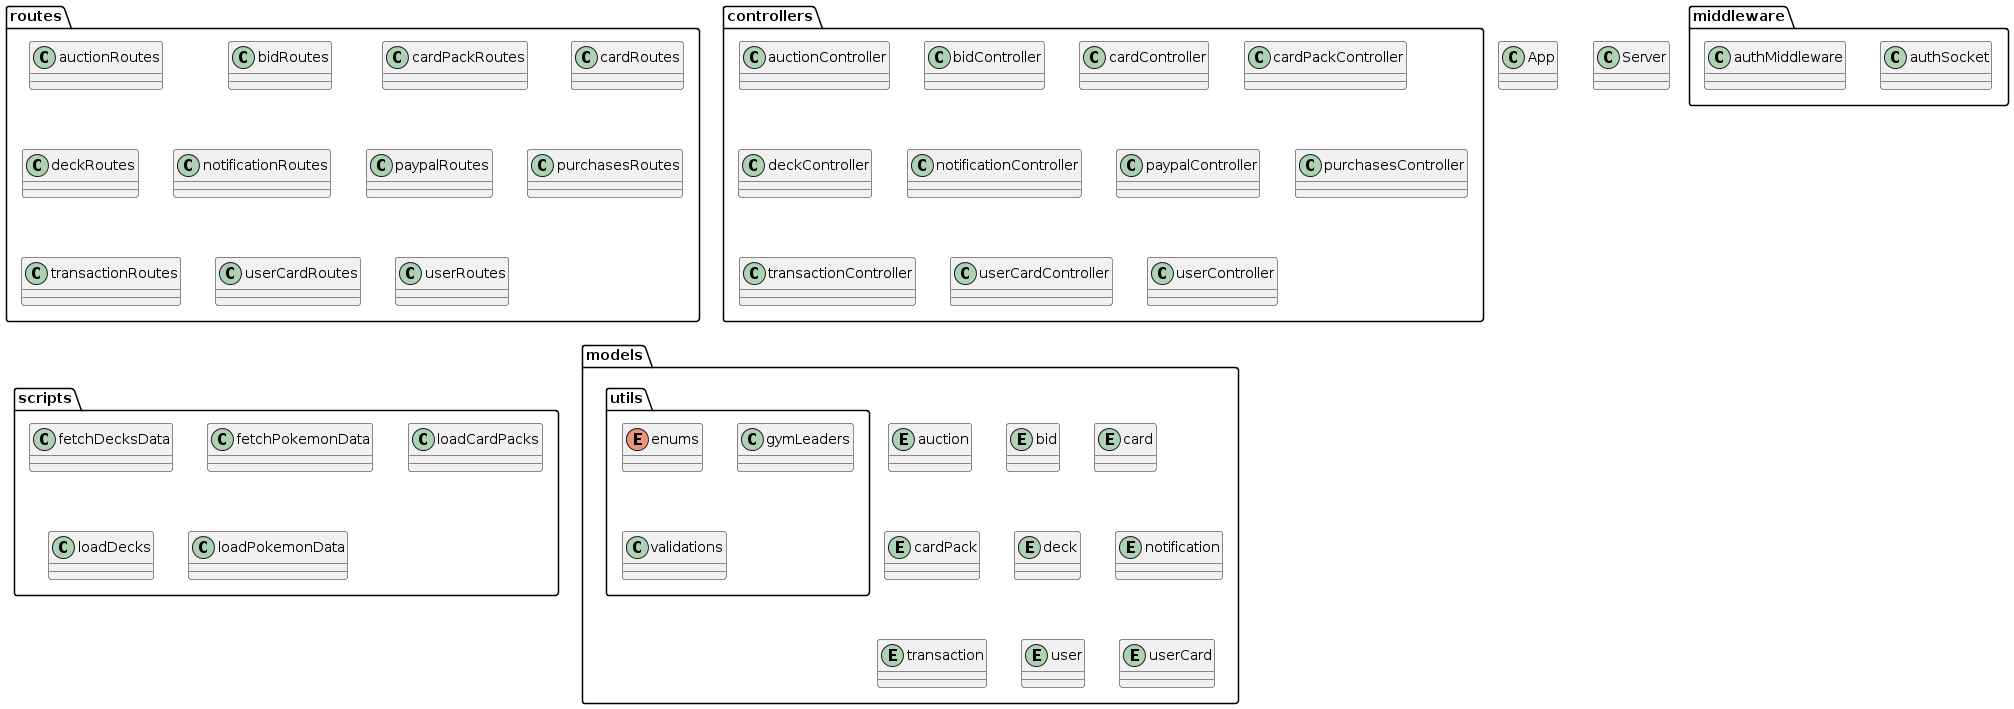
\includegraphics[width=1\linewidth]{figures/6-Analisis/6-Clases/6_6_Clases-restapi.png}
    \caption{Diagrama de Clases del Paquete restapi}
    \label{fig:6_6_Diagrama-Clases}
\end{figure}


\subsection{Descripción de las Clases} \hypertarget{sec:6_6_3-Descripcion-Clases}{} \label{sec:6_6_3-Descripcion-Clases}
A continuación, se describen las clases que componen el sistema y las relaciones entre ellas.
\subsubsection{Clase \textit{server}}

\subsubsection{Descripción de Clase. Server} \label{sec:descripcion_server}
\begin{longtable}{
    >{\columncolor{lightgreen!20}}p{4cm}
    p{12cm}
    }
    \caption{Descripción de Clase. Server} \label{table:descripcion_server} \\
    \toprule
    \rowcolor{darkgreen!50}
    \textbf{Clase} & \multicolumn{1}{>{\columncolor{darkgreen!50}\centering\arraybackslash}p{12cm}}{\textbf{SERVER}} \\
    \endfirsthead
    
    \multicolumn{2}{c}%
    {{ \tablename\ \thetable{} Descripción de Clase. Server -- continuación de la página anterior}} \\
    \toprule
    \rowcolor{darkgreen!50}
    \textbf{Clase} & \multicolumn{1}{>{\columncolor{darkgreen!50}\centering\arraybackslash}p{12cm}}{\textbf{SERVER}} \\
    \midrule
    \endhead
    
    \midrule
    \multicolumn{2}{r}{{Continúa en la siguiente página...}} \\ 
    \endfoot
    
    \bottomrule
    \endlastfoot
    
    \midrule
    Descripción & Esta clase configura y gestiona los servidores HTTP y HTTPS, la conexión a MongoDB, y la gestión de conexiones de sockets mediante Socket.IO. También incluye la configuración de variables de entorno y el manejo de errores. \\
    \midrule
    Atributos & \begin{itemize}[nosep,leftmargin=*]
      \item \textbf{httpPort}: number, puerto en el que el servidor HTTP escucha.
      \item \textbf{httpsPort}: number, puerto en el que el servidor HTTPS escucha (solo en producción).
      \item \textbf{mongoURI}: string, URI de conexión a la base de datos MongoDB.
      \item \textbf{httpsOptions}: object, opciones para el servidor HTTPS en producción.
      \item \textbf{httpServer}: object, instancia del servidor HTTP.
      \item \textbf{httpsServer}: object, instancia del servidor HTTPS.
      \item \textbf{io}: object, instancia de Socket.IO para manejar conexiones de sockets.
    \end{itemize} \\
    \midrule
    Métodos & \begin{itemize}[nosep,leftmargin=*]
      \item \textbf{config()}: void, configura las variables de entorno.
      \item \textbf{createServers()}: void, crea y configura los servidores HTTP y HTTPS.
      \item \textbf{connectToDatabase()}: void, conecta a la base de datos MongoDB.
      \item \textbf{startServers()}: void, inicia los servidores HTTP y HTTPS.
      \item \textbf{setupSocketIO()}: void, configura el middleware de autenticación de sockets y maneja eventos de conexión y desconexión.
      \item \textbf{closeServer()}: Promise<void>, cierra los servidores HTTP, HTTPS y la conexión a la base de datos.
    \end{itemize} \\
    \midrule
    Relaciones & \begin{itemize}[nosep,leftmargin=*]
      \item \textbf{App}: Importa y usa la clase App.
      \item \textbf{AuthSocket}: Importa y usa el middleware de autenticación de sockets.
    \end{itemize} \\
    \end{longtable}

\subsubsection{Clase \textit{app}}
\subsubsection{Descripción de Clase. App} \label{sec:descripcion_app}
\begin{longtable}{
    >{\columncolor{lightgreen!20}}p{4cm}
    p{12cm}
    }
    \caption{Descripción de Clase. App} \label{table:descripcion_app} \\
    \toprule
    \rowcolor{darkgreen!50}
    \textbf{Clase} & \multicolumn{1}{>{\columncolor{darkgreen!50}\centering\arraybackslash}p{12cm}}{\textbf{APP}} \\
    \endfirsthead
    
    \multicolumn{2}{c}%
    {{ \tablename\ \thetable{} Descripción de Clase. App -- continuación de la página anterior}} \\
    \toprule
    \rowcolor{darkgreen!50}
    \textbf{Clase} & \multicolumn{1}{>{\columncolor{darkgreen!50}\centering\arraybackslash}p{12cm}}{\textbf{APP}} \\
    \midrule
    \endhead
    
    \midrule
    \multicolumn{2}{r}{{Continúa en la siguiente página...}} \\ 
    \endfoot
    
    \bottomrule
    \endlastfoot
    
    \midrule
    Descripción & Esta clase configura y gestiona la aplicación Express, incluyendo las políticas CORS, las rutas de la API y el middleware para el manejo de errores. \\
    \midrule
    Atributos & \begin{itemize}[nosep,leftmargin=*]
      \item \textbf{app}: Application, instancia de la aplicación Express.
    \end{itemize} \\
    \midrule
    Métodos & \begin{itemize}[nosep,leftmargin=*]
      \item \textbf{use()}: void, permite configurar las rutas y los middlewares de la aplicación.
      \item \textbf{listen()}: void, inicia el servidor en el puerto especificado.
      \item \textbf{errorHandler()}: void, middleware para manejar errores en la aplicación.
    \end{itemize} \\
    \midrule
    Relaciones & \begin{itemize}[nosep,leftmargin=*]
      \item \textbf{AuctionRouter}: Importa y usa las rutas de subasta.
      \item \textbf{BidRouter}: Importa y usa las rutas de oferta.
      \item \textbf{CardPackRouter}: Importa y usa las rutas de paquetes de cartas.
      \item \textbf{CardRouter}: Importa y usa las rutas de cartas.
      \item \textbf{DeckRouter}: Importa y usa las rutas de mazos.
      \item \textbf{NotificationRouter}: Importa y usa las rutas de notificaciones.
      \item \textbf{PaypalRouter}: Importa y usa las rutas de PayPal.
      \item \textbf{PurchasesRouter}: Importa y usa las rutas de compras.
      \item \textbf{TransactionRouter}: Importa y usa las rutas de transacciones.
      \item \textbf{UserCardRouter}: Importa y usa las rutas de cartas de usuario.
      \item \textbf{UserRouter}: Importa y usa las rutas de usuario.
    \end{itemize} \\
    \end{longtable}


\subsubsection{Clases del paquete \textit{middlewares}}
\subsubsubsection{Descripción de Clase. AuthMiddleware} \label{sec:descripcion_authmiddleware}
\begin{longtable}{
    >{\columncolor{lightgreen!20}}p{4cm}
    p{12cm}
    }
    \caption{Descripción de Clase. AuthMiddleware} \label{table:descripcion_authmiddleware} \\
    \toprule
    \rowcolor{darkgreen!50}
    \textbf{Clase} & \multicolumn{1}{>{\columncolor{darkgreen!50}\centering\arraybackslash}p{12cm}}{\textbf{AUTHMIDDLEWARE}} \\
    \endfirsthead
    
    \multicolumn{2}{c}%
    {{ \tablename\ \thetable{} Descripción de Clase. AuthMiddleware -- continuación de la página anterior}} \\
    \toprule
    \rowcolor{darkgreen!50}
    \textbf{Clase} & \multicolumn{1}{>{\columncolor{darkgreen!50}\centering\arraybackslash}p{12cm}}{\textbf{AUTHMIDDLEWARE}} \\
    \midrule
    \endhead
    
    \midrule
    \multicolumn{2}{r}{{Continúa en la siguiente página...}} \\ 
    \endfoot
    
    \bottomrule
    \endlastfoot
    
    \midrule
    Descripción & Esta clase proporciona middleware para la autenticación y autorización de usuarios mediante tokens JWT. Incluye la verificación de tokens y la verificación de roles de administrador. \\
    \midrule
    Atributos & \begin{itemize}[nosep,leftmargin=*]
      \item \textbf{jwt}: Object, módulo para manejar JSON Web Tokens.
    \end{itemize} \\
    \midrule
    Métodos & \begin{itemize}[nosep,leftmargin=*]
      \item \textbf{auth(req: Request, res: Response, next: any)}: void, middleware para verificar la autenticidad del token JWT en las peticiones.
      \item \textbf{verifyAdmin(req: Request, res: Response, next: any)}: void, middleware para verificar que el usuario tiene rol de administrador.
    \end{itemize} \\
    \midrule
    Relaciones & \\
    \end{longtable}

\subsubsubsection{Descripción de Clase. AuthSocket} \label{sec:descripcion_authsocket}
\begin{longtable}{
    >{\columncolor{lightgreen!20}}p{4cm}
    p{12cm}
    }
    \caption{Descripción de Clase. AuthSocket} \label{table:descripcion_authsocket} \\
    \toprule
    \rowcolor{darkgreen!50}
    \textbf{Clase} & \multicolumn{1}{>{\columncolor{darkgreen!50}\centering\arraybackslash}p{12cm}}{\textbf{AUTHSOCKET}} \\
    \endfirsthead
    
    \multicolumn{2}{c}%
    {{ \tablename\ \thetable{} Descripción de Clase. AuthSocket -- continuación de la página anterior}} \\
    \toprule
    \rowcolor{darkgreen!50}
    \textbf{Clase} & \multicolumn{1}{>{\columncolor{darkgreen!50}\centering\arraybackslash}p{12cm}}{\textbf{AUTHSOCKET}} \\
    \midrule
    \endhead
    
    \midrule
    \multicolumn{2}{r}{{Continúa en la siguiente página...}} \\ 
    \endfoot
    
    \bottomrule
    \endlastfoot
    
    \midrule
    Descripción & Esta clase proporciona middleware para la autenticación de conexiones de sockets mediante tokens JWT. Verifica la validez y el formato del token proporcionado en el handshake de la conexión del socket. \\
    \midrule
    Atributos & \begin{itemize}[nosep,leftmargin=*]
      \item \textbf{jwt}: Object, módulo para manejar JSON Web Tokens.
    \end{itemize} \\
    \midrule
    Métodos & \begin{itemize}[nosep,leftmargin=*]
      \item \textbf{authSocket(socket: Socket, next: (err?: Error) => void)}: void, middleware para verificar la autenticidad del token JWT en las conexiones de sockets.
    \end{itemize} \\
    \midrule
    Relaciones &  \\
    \end{longtable}


\subsubsection{Clases del paquete \textit{routes}}
\subsubsubsection{Descripción de Clase. AuctionRouter} \label{sec:descripcion_auctionrouter}
\begin{longtable}{
    >{\columncolor{lightgreen!20}}p{4cm}
    p{12cm}
    }
    \caption{Descripción de Clase. AuctionRouter} \label{table:descripcion_auctionrouter} \\
    \toprule
    \rowcolor{darkgreen!50}
    \textbf{Clase} & \multicolumn{1}{>{\columncolor{darkgreen!50}\centering\arraybackslash}p{12cm}}{\textbf{AUCTIONROUTER}} \\
    \endfirsthead
    
    \multicolumn{2}{c}%
    {{ \tablename\ \thetable{} Descripción de Clase. AuctionRouter -- continuación de la página anterior}} \\
    \toprule
    \rowcolor{darkgreen!50}
    \textbf{Clase} & \multicolumn{1}{>{\columncolor{darkgreen!50}\centering\arraybackslash}p{12cm}}{\textbf{AUCTIONROUTER}} \\
    \midrule
    \endhead
    
    \midrule
    \multicolumn{2}{r}{{Continúa en la siguiente página...}} \\ 
    \endfoot
    
    \bottomrule
    \endlastfoot
    
    \midrule
    Descripción & Esta clase configura y gestiona las rutas relacionadas con las subastas en la aplicación Express. Incluye la autenticación mediante middleware y validaciones para las peticiones. \\
    \midrule
    Atributos & \begin{itemize}[nosep,leftmargin=*]
      \item \textbf{auctionRouter}: Router, instancia del enrutador de Express para las subastas.
    \end{itemize} \\
    \midrule
    Métodos & \begin{itemize}[nosep,leftmargin=*]
      \item \textbf{getAuctions(req: Request, res: Response)}: void, maneja la obtención de todas las subastas.
      \item \textbf{getAuction(req: Request, res: Response)}: void, maneja la obtención de una subasta por su ID.
      \item \textbf{getActiveAuctions(req: Request, res: Response)}: void, maneja la obtención de todas las subastas activas.
      \item \textbf{getActiveAuctionsByUser(req: Request, res: Response)}: void, maneja la obtención de todas las subastas activas de un usuario.
      \item \textbf{putUserCardUpForAuction(req: Request, res: Response)}: void, maneja la puesta en subasta de una carta de usuario.
      \item \textbf{withdrawnUserCardFromAuction(req: Request, res: Response)}: void, maneja la retirada de una carta de usuario de una subasta.
      \item \textbf{checkAllActiveAuctions(req: Request, res: Response)}: void, verifica todas las subastas activas y actualiza su estado si es necesario.
    \end{itemize} \\
    \midrule
    Relaciones & \begin{itemize}[nosep,leftmargin=*]
      \item \textbf{AuthMiddleware}: Middleware para la autenticación de usuarios.
      \item \textbf{AuctionController}: Importa y utiliza métodos del controlador de subastas.
    \end{itemize} \\
    \end{longtable}

    \subsubsubsection{Descripción de Clase. BidRouter} \label{sec:descripcion_bidrouter}
\begin{longtable}{
    >{\columncolor{lightgreen!20}}p{4cm}
    p{12cm}
    }
    \caption{Descripción de Clase. BidRouter} \label{table:descripcion_bidrouter} \\
    \toprule
    \rowcolor{darkgreen!50}
    \textbf{Clase} & \multicolumn{1}{>{\columncolor{darkgreen!50}\centering\arraybackslash}p{12cm}}{\textbf{BIDROUTER}} \\
    \endfirsthead
    
    \multicolumn{2}{c}%
    {{ \tablename\ \thetable{} Descripción de Clase. BidRouter -- continuación de la página anterior}} \\
    \toprule
    \rowcolor{darkgreen!50}
    \textbf{Clase} & \multicolumn{1}{>{\columncolor{darkgreen!50}\centering\arraybackslash}p{12cm}}{\textbf{BIDROUTER}} \\
    \midrule
    \endhead
    
    \midrule
    \multicolumn{2}{r}{{Continúa en la siguiente página...}} \\ 
    \endfoot
    
    \bottomrule
    \endlastfoot
    
    \midrule
    Descripción & Esta clase configura y gestiona las rutas relacionadas con las pujas en la aplicación Express. Incluye la autenticación mediante middleware y validaciones para las peticiones. \\
    \midrule
    Atributos & \begin{itemize}[nosep,leftmargin=*]
      \item \textbf{bidRouter}: Router, instancia del enrutador de Express para las pujas.
    \end{itemize} \\
    \midrule
    Métodos & \begin{itemize}[nosep,leftmargin=*]
      \item \textbf{getBidById(req: Request, res: Response)}: void, maneja la obtención de una puja por su ID.
      \item \textbf{createBid(req: Request, res: Response)}: void, maneja la creación de una nueva puja.
      \item \textbf{getActiveBidsByUser(req: Request, res: Response)}: void, maneja la obtención de todas las pujas activas de un usuario.
      \item \textbf{withdrawBid(req: Request, res: Response)}: void, maneja la retirada de una puja.
    \end{itemize} \\
    \midrule
    Relaciones & \begin{itemize}[nosep,leftmargin=*]
      \item \textbf{AuthMiddleware}: Middleware para la autenticación de usuarios.
      \item \textbf{BidController}: Importa y utiliza métodos del controlador de pujas.
    \end{itemize} \\
    \end{longtable}

\subsubsubsection{Descripción de Clase. CardPackRouter} \label{sec:descripcion_cardpackrouter}
\begin{longtable}{
    >{\columncolor{lightgreen!20}}p{4cm}
    p{12cm}
    }
    \caption{Descripción de Clase. CardPackRouter} \label{table:descripcion_cardpackrouter} \\
    \toprule
    \rowcolor{darkgreen!50}
    \textbf{Clase} & \multicolumn{1}{>{\columncolor{darkgreen!50}\centering\arraybackslash}p{12cm}}{\textbf{CARDPACKROUTER}} \\
    \endfirsthead
    
    \multicolumn{2}{c}%
    {{ \tablename\ \thetable{} Descripción de Clase. CardPackRouter -- continuación de la página anterior}} \\
    \toprule
    \rowcolor{darkgreen!50}
    \textbf{Clase} & \multicolumn{1}{>{\columncolor{darkgreen!50}\centering\arraybackslash}p{12cm}}{\textbf{CARDPACKROUTER}} \\
    \midrule
    \endhead
    
    \midrule
    \multicolumn{2}{r}{{Continúa en la siguiente página...}} \\ 
    \endfoot
    
    \bottomrule
    \endlastfoot
    
    \midrule
    Descripción & Esta clase configura y gestiona las rutas relacionadas con los sobres de cartas en la aplicación Express. Incluye la autenticación mediante middleware. \\
    \midrule
    Atributos & \begin{itemize}[nosep,leftmargin=*]
      \item \textbf{cardPackRouter}: Router, instancia del enrutador de Express para los sobres de cartas.
    \end{itemize} \\
    \midrule
    Métodos & \begin{itemize}[nosep,leftmargin=*]
      \item \textbf{getCardPacks(req: Request, res: Response)}: void, maneja la obtención de todos los sobres de cartas.
    \end{itemize} \\
    \midrule
    Relaciones & \begin{itemize}[nosep,leftmargin=*]
      \item \textbf{AuthMiddleware}: Middleware para la autenticación de usuarios.
      \item \textbf{CardPackController}: Importa y utiliza el método del controlador de sobres de cartas.
    \end{itemize} \\
    \end{longtable}


\subsubsubsection{Descripción de Clase. CardRouter} \label{sec:descripcion_cardrouter}
\begin{longtable}{
    >{\columncolor{lightgreen!20}}p{4cm}
    p{12cm}
    }
    \caption{Descripción de Clase. CardRouter} \label{table:descripcion_cardrouter} \\
    \toprule
    \rowcolor{darkgreen!50}
    \textbf{Clase} & \multicolumn{1}{>{\columncolor{darkgreen!50}\centering\arraybackslash}p{12cm}}{\textbf{CARDROUTER}} \\
    \endfirsthead
    
    \multicolumn{2}{c}%
    {{ \tablename\ \thetable{} Descripción de Clase. CardRouter -- continuación de la página anterior}} \\
    \toprule
    \rowcolor{darkgreen!50}
    \textbf{Clase} & \multicolumn{1}{>{\columncolor{darkgreen!50}\centering\arraybackslash}p{12cm}}{\textbf{CARDROUTER}} \\
    \midrule
    \endhead
    
    \midrule
    \multicolumn{2}{r}{{Continúa en la siguiente página...}} \\ 
    \endfoot
    
    \bottomrule
    \endlastfoot
    
    \midrule
    Descripción & Esta clase configura y gestiona las rutas relacionadas con las cartas en la aplicación Express. Incluye la autenticación mediante middleware y validaciones para las peticiones. \\
    \midrule
    Atributos & \begin{itemize}[nosep,leftmargin=*]
      \item \textbf{cardRouter}: Router, instancia del enrutador de Express para las cartas.
    \end{itemize} \\
    \midrule
    Métodos & \begin{itemize}[nosep,leftmargin=*]
      \item \textbf{getCard(req: Request, res: Response)}: void, maneja la obtención de una carta por su ID.
    \end{itemize} \\
    \midrule
    Relaciones & \begin{itemize}[nosep,leftmargin=*]
      \item \textbf{AuthMiddleware}: Middleware para la autenticación de usuarios.
      \item \textbf{CardController}: Importa y utiliza el método del controlador de cartas.
    \end{itemize} \\
    \end{longtable}

\subsubsubsection{Descripción de Clase. NotificationRouter} \label{sec:descripcion_notificationrouter}
\begin{longtable}{
    >{\columncolor{lightgreen!20}}p{4cm}
    p{12cm}
    }
    \caption{Descripción de Clase. NotificationRouter} \label{table:descripcion_notificationrouter} \\
    \toprule
    \rowcolor{darkgreen!50}
    \textbf{Clase} & \multicolumn{1}{>{\columncolor{darkgreen!50}\centering\arraybackslash}p{12cm}}{\textbf{NOTIFICATIONROUTER}} \\
    \endfirsthead
    
    \multicolumn{2}{c}%
    {{ \tablename\ \thetable{} Descripción de Clase. NotificationRouter -- continuación de la página anterior}} \\
    \toprule
    \rowcolor{darkgreen!50}
    \textbf{Clase} & \multicolumn{1}{>{\columncolor{darkgreen!50}\centering\arraybackslash}p{12cm}}{\textbf{NOTIFICATIONROUTER}} \\
    \midrule
    \endhead
    
    \midrule
    \multicolumn{2}{r}{{Continúa en la siguiente página...}} \\ 
    \endfoot
    
    \bottomrule
    \endlastfoot
    
    \midrule
    Descripción & Esta clase configura y gestiona las rutas relacionadas con las notificaciones en la aplicación Express. Incluye la autenticación mediante middleware y validaciones para las peticiones. \\
    \midrule
    Atributos & \begin{itemize}[nosep,leftmargin=*]
      \item \textbf{notificationRouter}: Router, instancia del enrutador de Express para las notificaciones.
    \end{itemize} \\
    \midrule
    Métodos & \begin{itemize}[nosep,leftmargin=*]
      \item \textbf{getNotifications(req: Request, res: Response)}: void, maneja la obtención de todas las notificaciones de un usuario.
      \item \textbf{markAsRead(req: Request, res: Response)}: void, maneja el marcado de una notificación como leída.
      \item \textbf{markAllAsRead(req: Request, res: Response)}: void, maneja el marcado de todas las notificaciones de un usuario como leídas.
      \item \textbf{hasUnreadNotifications(req: Request, res: Response)}: void, verifica si un usuario tiene notificaciones no leídas.
    \end{itemize} \\
    \midrule
    Relaciones & \begin{itemize}[nosep,leftmargin=*]
      \item \textbf{AuthMiddleware}: Middleware para la autenticación de usuarios.
      \item \textbf{NotificationController}: Importa y utiliza métodos del controlador de notificaciones.
    \end{itemize} \\
    \end{longtable}

    \subsubsubsection{Descripción de Clase. PaypalRouter} \label{sec:descripcion_paypalrouter}
\begin{longtable}{
    >{\columncolor{lightgreen!20}}p{4cm}
    p{12cm}
    }
    \caption{Descripción de Clase. PaypalRouter} \label{table:descripcion_paypalrouter} \\
    \toprule
    \rowcolor{darkgreen!50}
    \textbf{Clase} & \multicolumn{1}{>{\columncolor{darkgreen!50}\centering\arraybackslash}p{12cm}}{\textbf{PAYPALROUTER}} \\
    \endfirsthead
    
    \multicolumn{2}{c}%
    {{ \tablename\ \thetable{} Descripción de Clase. PaypalRouter -- continuación de la página anterior}} \\
    \toprule
    \rowcolor{darkgreen!50}
    \textbf{Clase} & \multicolumn{1}{>{\columncolor{darkgreen!50}\centering\arraybackslash}p{12cm}}{\textbf{PAYPALROUTER}} \\
    \midrule
    \endhead
    
    \midrule
    \multicolumn{2}{r}{{Continúa en la siguiente página...}} \\ 
    \endfoot
    
    \bottomrule
    \endlastfoot
    
    \midrule
    Descripción & Esta clase configura y gestiona las rutas relacionadas con las órdenes de PayPal en la aplicación Express. Incluye validaciones para las peticiones y manejo de errores. \\
    \midrule
    Atributos & \begin{itemize}[nosep,leftmargin=*]
      \item \textbf{paypalRouter}: Router, instancia del enrutador de Express para las órdenes de PayPal.
    \end{itemize} \\
    \midrule
    Métodos & \begin{itemize}[nosep,leftmargin=*]
      \item \textbf{createOrder(req: Request, res: Response)}: void, maneja la creación de una nueva orden de PayPal.
      \item \textbf{updateOrder(req: Request, res: Response)}: void, maneja la actualización del saldo de un usuario después de completar un pago.
    \end{itemize} \\
    \midrule
    Relaciones & \begin{itemize}[nosep,leftmargin=*]
      \item \textbf{PaypalController}: Importa y utiliza el método del controlador de PayPal para crear órdenes.
      \item \textbf{User}: Importa y utiliza el modelo de usuario para actualizar el saldo.
    \end{itemize} \\
    \end{longtable}


\subsubsection{Clases del paquete \textit{controllers}}
\subsubsection{Clases del paquete \textit{models}}
\subsubsection{Clases del paquete \textit{utils}}
\subsubsection{Clases del paquete \textit{scripts}}

